\chapter{Lie algebras}
\section{left-invariant vector fields}
\begin{itemize}
	\item vector field $\bar{A}$ is invariant under push-forward, $L_{g *}: V_h \rightarrow V_{g h}, \forall h$,
	\begin{equation}
		(L_{g *} \bar{A}) \big|_{g h} = \bar{A} \big|_{g h}
	\end{equation}
	i.e.,
	\begin{equation}
		\bar{A}(x^i) \big|_h = \bar{A}(y^i) \big|_{g h}
	\end{equation}
	where $L_g^* y^i = x^i \iff y^i(g h) = x^i(h)$.
	
	\item see appendix \ref{B}, maps between manifolds.
	
	\item the set of all left invariant vector filed is denoted by $\mathfrak{g}$, and $\mathfrak{g} \simeq V_e$.
\end{itemize}

\section{Lie algebras}
\begin{itemize}
	\item $A \equiv \bar{A}_e$ and $\bar{A}_g = L_{g *} A, \forall g$.
	
	\item a vector space, $V$, along with Lie bracket, $[,]: V \times V \rightarrow V$, is a \textbf{Lie algebra},
	\begin{itemize}
		\item $[A, B] = - [B, A]$.
		
		\item Jacob identity, $[A, [B, C]] + [C, [A, B]] + [B, [C, A]] = 0$.
	\end{itemize}
	
	\item for a Lie group $G$, its Lie bracket is the commutator,
	\begin{equation}
		[\bar{A}, \bar{B}]^a = \bar{A}^b \nabla_b \bar{B}^a - \bar{B}^b \nabla_b \bar{A}^a
	\end{equation}
	\begin{itemize}
		\item $L_{g *} [\bar{A}, \bar{B}] = [L_{g *} \bar{A}, L_{g *} \bar{B}] = [\bar{A}, \bar{B}] \in \mathfrak{g}$.
		
		\begin{tcolorbox}[title=proof:]
			\begin{align}
				L_{g *} [\bar{A}, \bar{B}] &= L_{g *} \Big( \frac{\partial}{\partial x^i} \Big|_h \Big) \Big( A^j \frac{\partial}{\partial x^j} B^i - B^j \frac{\partial}{\partial x^j} A^i \Big) \Big|_{h, x} \notag \\
				&= \Big( \frac{\partial}{\partial y^i} \Big|_{g h} \Big) \Big( A^j \frac{\partial}{\partial x^j} B^i - B^j \frac{\partial}{\partial x^j} A^i \Big) \Big|_{h, x}
			\end{align}
			notice that for left-invariant v. f. as a scalar field, $(L_g^* A^i \big|_y) \big|_h = A^i \big|_{g h, y}$ and,
			\begin{align}
				& \Big( \frac{\partial}{\partial x^j} A^i \Big) \Big|_{h, x} \equiv \Big( \frac{\partial}{\partial x^j} \Big) \Big|_h (L_g^* A^i \Big|_y) \Big|_h = L_{g *} \Big( \frac{\partial}{\partial x^j} \Big|_h \Big) (A^i \Big|_{g h, y}) \notag \\
				\Longrightarrow & \Big( \frac{\partial}{\partial x^j} A^i \Big) \Big|_{h, x} = \Big( \frac{\partial}{\partial y^j} A^i \Big) \Big|_{g h, y}
			\end{align}
			
			so $L_{g *} [\bar{A}, \bar{B}] = [\bar{A}, \bar{B}]$.
		\end{tcolorbox}
		
		\item satisfies the Jacob identity.
		
		\begin{tcolorbox}[title=proof:]
			\begin{align}
				& [A, [B, C]] + [C, [A, B]] + [B, [C, A]] \notag \\
				= & A^c \partial_c (B^b \partial_b C^a - C^b \partial_b B^a) - (B^c \partial_c C^b - C^c \partial_c B^b) \partial_b A^a + \cdots \notag \\
				= & \mathcolor{red}{A^c \partial_c (B^b) \partial_b C^a} \mathcolor{blue}{+ A^c B^b \partial_c \partial_b C^a} \mathcolor{red}{- A^c \partial_c (C^b) \partial_b B^a} \mathcolor{blue}{+ A^c C^b \partial_c \partial_b B^a} \notag \\
				& \mathcolor{red}{- B^c \partial_c (C^b) \partial_b A^a + C^c \partial_c (B^b) \partial_b A^a} \notag \\
				& \mathcolor{red}{+ (B \partial C \partial A - B \partial A \partial C - C \partial A \partial B + A \partial C \partial B)} \notag \\
				& \mathcolor{blue}{+ (B C \partial \partial A - B A \partial \partial C)} \notag \\
				& \mathcolor{red}{+ (C \partial A \partial B - C \partial B \partial A - A \partial B \partial C + B \partial A \partial C)} \notag \\
				& \mathcolor{blue}{+ (C A \partial \partial B - C B \partial \partial A)} = 0
			\end{align}
		\end{tcolorbox}
	\end{itemize}
	
	\noindent\rule[0.5ex]{\linewidth}{0.5pt} % horizontal line
	
	\item \textbf{def.:} the \textbf{Lie algebra direct sum} of two Lie algebras, $\mathfrak{g}_1, \mathfrak{g}_2$, is the \textbf{vector space direct sum} (i.e. $\mathfrak{g}_1, \mathfrak{g}_2$ are \colorbox{yellow}{linearly independent $\iff \mathfrak{g}_1 \cap \mathfrak{g}_2 = \{0\}$}), $\mathfrak{g} = \mathfrak{g}_1 \oplus \mathfrak{g}_2$, with the Lie bracket defined to be,
	\begin{align}
		[\cdot, \cdot] : \mathfrak{g} \times \mathfrak{g} & \rightarrow \mathfrak{g} \notag \\
		[A_1 + A_2, B_1 + B_2] &= [A_1, B_1] + [A_2, B_2] \quad \forall A_1, B_1 \in \mathfrak{g}_1, A_2, B_2 \in \mathfrak{g}_2
	\end{align}
	i.e. we define the Lie bracket in the way that $[\mathfrak{g}_1, \mathfrak{g}_2] = \{0\}$.
\end{itemize}

\subsection{subalgebras, ideals \& simple, solvable, nilpotent Lie algebras} \label{3.2.1}
\begin{itemize}
	\item \textbf{def.:} \textbf{subalgebra} $\mathfrak{h} \subset \mathfrak{g}$ is a subspace, satisfying that $[\mathfrak{h}, \mathfrak{h}] \subseteq \mathfrak{h}$.
	\begin{itemize}
		\item \textbf{def.:} Abelian subalgebra $\mathfrak{h}$ is a subalgebra, satisfying that $[A, B] = 0, \forall A, B \in \mathfrak{h}$.
	\end{itemize}
	
	\item \textbf{def.:} invariant subalgebra (i.e. \textbf{ideal}) $\mathfrak{h}$ is a subalgebra, satisfying that $[\mathfrak{h}, \mathfrak{g}] \subseteq \mathfrak{h}$.
	\begin{itemize}
		\item Abelian ideal.
		
		\item proper invariant subalgebra (also called \textbf{proper ideal}) is an ideal that is not $\mathfrak{g}, \{0\}$.
		
		\item trivial subalgebras are $\mathfrak{g}, \{0\}$.
	\end{itemize}
	
	\noindent\rule[0.5ex]{\linewidth}{0.5pt} % horizontal line
	
	\item Lie algebra decomposes as the direct sum of its ideals, $\mathfrak{h}_1, \mathfrak{h}_2, \cdots$, i.e.,
	\begin{equation}
		\mathfrak{g} = \mathfrak{h}_1 \oplus \mathfrak{h}_2 \oplus \cdots
	\end{equation}
	then $\oplus$ is called \textbf{Lie algebra direct sum}.
	
	\begin{tcolorbox}[title=proof:]
		by def., $[\mathfrak{h}_i, \mathfrak{h}_j] \subseteq \mathfrak{h}_i \cap \mathfrak{h}_j = \{0\}$, if $i \neq j$.
	\end{tcolorbox}
	
	\noindent\rule[0.5ex]{\linewidth}{0.5pt} % horizontal line
	
	\item \textbf{def.:} a Lie algebra \textbf{without nontrivial ideal} is \textbf{irreducible}.
	\begin{itemize}
		\item all 1-dim. Lie algebras are irreducible.
	\end{itemize}
	
	\item \textbf{def.:} a \textbf{irreducible} Lie algebra with $\dim \mathfrak{g} \geq 2$ is \textbf{simple}.
	\begin{itemize}
		\item equivalent \textbf{def.:} irreducible non-Abelian Lie algebras are simple.
		
		\begin{tcolorbox}[title=proof:]
			all the subspaces of an Abelian Lie algebra is its ideal $\Longrightarrow$ Abelian Lie algebras aren't irreducible unless $\dim = 1$, so,
			
			\begin{figure}[H]
				\centering
				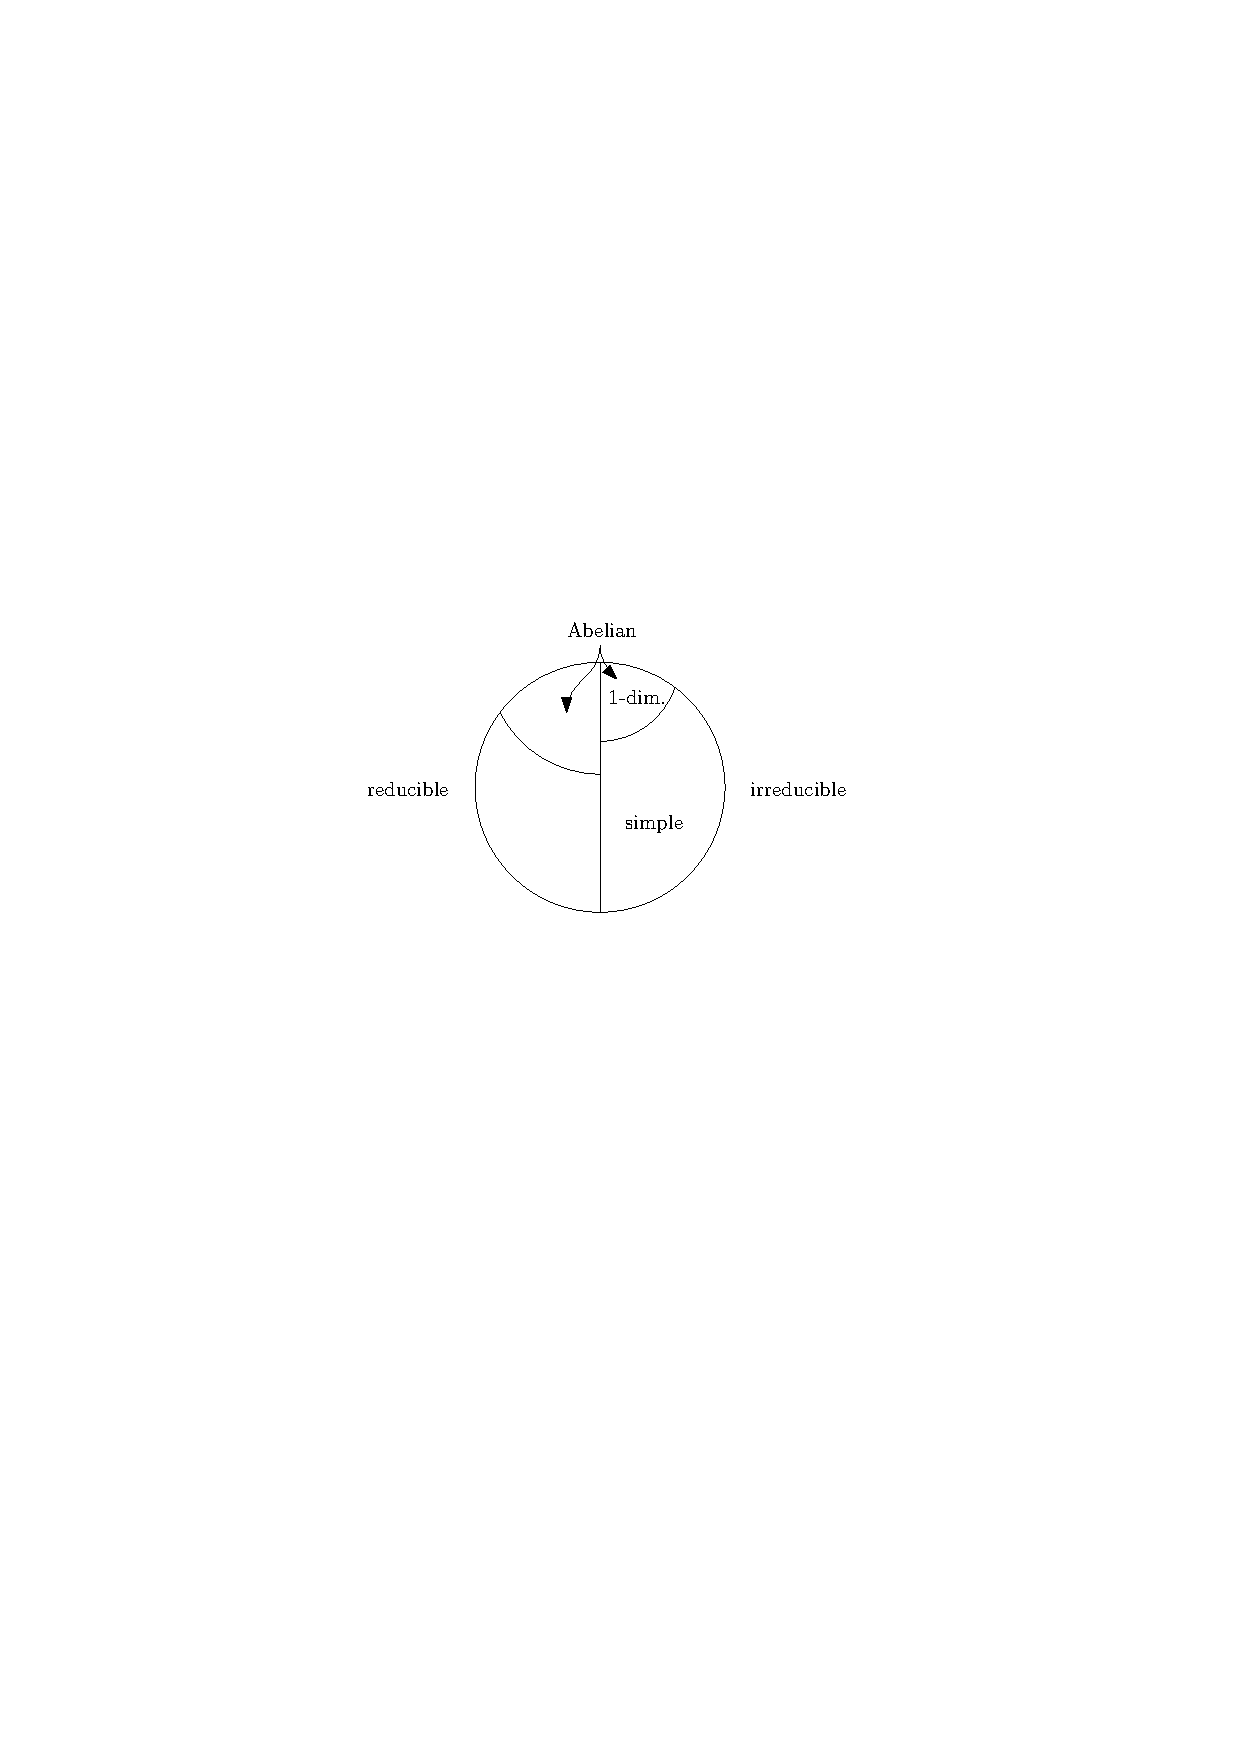
\includegraphics[scale=1]{figures/(non-)Abelian, (ir)reducible, and simple.pdf}
				\caption{(non-)Abelian, (ir)reducible, and simple Lie algebras}
			\end{figure}
		\end{tcolorbox}
	\end{itemize}
	
	\item \textbf{def.:} a Lie algebra $\mathfrak{g}$ is \textbf{solvable} if $\mathfrak{g}_i = \{0\}$ for some $i$, where,
	\begin{equation}
		\mathfrak{g}_{i + 1} = [\mathfrak{g}_i, \mathfrak{g}_i] \quad \text{and} \quad \mathfrak{g}_0 = \mathfrak{g}
	\end{equation}
	\begin{itemize}
		\item $\mathfrak{g}_i$ is an ideal in $\mathfrak{g}_{i - 1}$, but not necessarily an ideal in $\mathfrak{g}$.
		
		\begin{tcolorbox}[title=proof:]
			$\forall A \in \mathfrak{g}_i \subseteq \mathfrak{g}_{i - 1}$ and $\forall B \in \mathfrak{g}_{i - 1}$, $[A, B] \in \mathfrak{g}_i$, which means $[\mathfrak{g}_i, \mathfrak{g}_{i - 1}] \subseteq \mathfrak{g}_i$.
		\end{tcolorbox}
	\end{itemize}
	
	\item \textbf{def.:} a Lie algebra $\mathfrak{g}$ is \textbf{nilpotent} if $\mathfrak{g}^i = \{0\}$ for some $i$, where,
	\begin{equation}
		\mathfrak{g}^{i + 1} = [\mathfrak{g}, \mathfrak{g}^i] \quad \text{and} \quad \mathfrak{g}^0 = \mathfrak{g}
	\end{equation}
	\begin{itemize}
		\item $\mathfrak{g}^{i + 1} \subseteq \mathfrak{g}^i$.
		
		\item $\mathfrak{g}^i$ is an ideal in $\mathfrak{g}$.
		
		\item nilpotent Lie algebra is solvable.
	\end{itemize}
\end{itemize}

\subsection{structure constants}
\begin{itemize}
	\item structure constants,
	\begin{align}
		& [X_i, X_j] = i \tensor{f}{_{i j}^k} X_k \iff [X_i, X_j]^a = i \tensor{f}{_{b c}^a} (X_i)^b (X_j)^c \\
		& [A_i, A_j] = - \tensor{f}{_{i j}^k} A_k \iff [A_i, A_j]^a = - \tensor{f}{_{b c}^a} (A_i)^b (A_j)^c
	\end{align}
	where $X_i = - i A_i$ are called the generators.
	\begin{itemize}
		\item if the generators are Hermitian, then the structure constants are real,
		\begin{equation}
			[X_i, X_j]^\dag = - i \tensor{f}{^*_{i j}^k} X_k = [X_j, X_i] = i \underbrace{\tensor{f}{_{j i}^k}}_{= - \tensor{f}{_{i j}^k}} X_k \Longrightarrow \tensor{f}{^*_{i j}^k} = \tensor{f}{_{i j}^k}
		\end{equation}
	\end{itemize}
\end{itemize}
